\section{Das Modell}
Im folgenden Abschnitt soll das in \ref{fig:ccmodel} gezeigte Modell zur Beschreibung von DNS-Cloud-Services detailliert erläutert werden. Dies soll zum Verständnis und als Hilfe bei der Anwendung dienen. Außerdem soll es die gewählte Darstellungsform und Notation beleuchten, die zur Erstellung des Modells genutzt wurde.

\begin{sidewaysfigure*}[ht]
    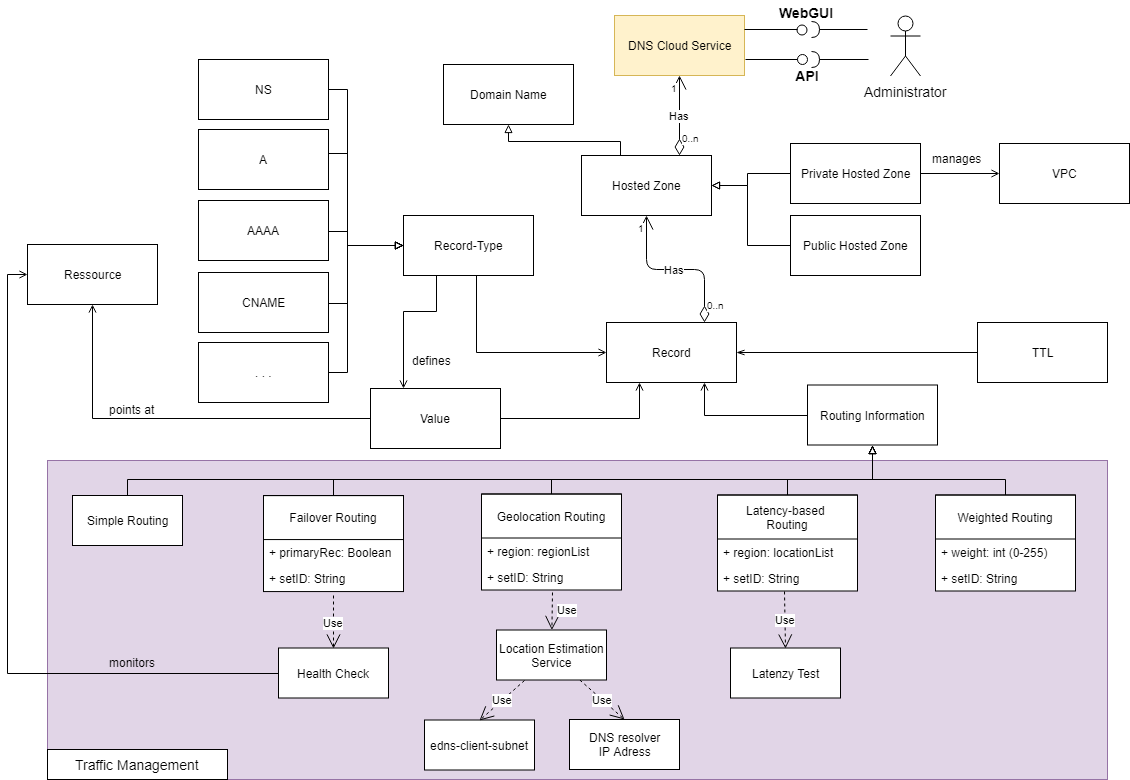
\includegraphics[width=\textwidth]{images/cc_modelxml.png}
    \caption{Modell zur Beschreibung von DNS-Cloud-Services}
    \label{fig:ccmodel}
\end{sidewaysfigure*}

\subsection{Schnittstellen}
Zur Nutzung der DNS-Cloud-Services allgemein stehen unterschiedliche Möglichkeiten zur Verfügung. Wird ein neues Benutzerkonto angelegt, geschieht dies über eine Weboberfläche. Nach der Einrichtung ist es möglich über die Benutzeroberfläche der Internetseite auf das Produktportfolio des Dienstleisters zuzugreifen. Sämtliche Interaktionen mit dem Cloud-Service sind über diese Weboberfläche möglich. So kann der Kunde jederzeit und von jedem internetfähigen Gerät, plattformunabhängig über den Browser seines Betriebssystems auf die Services zugreifen. Das bedeutet, dass keine Installation von zusätzlichen Anwendungen oder Treibern notwendig ist.

Eine weitere Möglichkeit ist der Zugriff über eine Schnittstelle zur Anwendungsprogrammierung (API). Diese Schnittstellen ermöglichen es mit der Hilfe von Kommandozeilenwerkzeugen auf die Services des Cloud-Providers zuzugreifen. Somit können auch ohne die Hilfe des Webinterfaces administrative Aufgaben bezüglich der Cloud erledigt werden. Eine API ermöglicht es ebenfalls über Skriptsprachen Routineaufgaben zu automatisieren oder den Cloud-Service in eine unternehmensinterne Software einzubinden. Dies bringt den Vorteil eines flexibleren Umgangs und einer bessere Einbindung des Cloud-Services in die alltäglichen Prozesse.

 \subsection{Hosted Zones}
Bei der Analyse der einzelnen DNS-Cloud-Dienstleistungen fällt auf, dass das zentrale Element die sogenannten Hosted-Zones darstellen. Sie dienen als Container zum Hosten der DNS-Einträge zu einer bestimmten Domäne und umschließen somit alle Informationen über die Weiterleitung des Datenverkehrs dieser.
Ein DNS-Cloud-Service kann über mehrere Hosted-Zones verfügen. Die Namensgebung findet hierbei meist über den Domain-Namen statt. Somit wird die Funktion der Hosted-Zones schnell ersichtlich. Außerdem ist über den Domain-Namen eine einzigartige Identifizierung der unterschiedlichen Zonen gewährleistet. Je nach DNS-Cloud-Dienstleistung kann jedoch auch ein abweichender Name zur betreffenden Domain gewählt werden. Laut den offiziellen Dokumenationen der Cloud-Provider, liegt das Limit an Hosted-Zones standardmäßig bei über 100 Hosted-Zones, bei allen drei untersuchten Anbietern.